\subsection{Robustness and uncertainty models}
    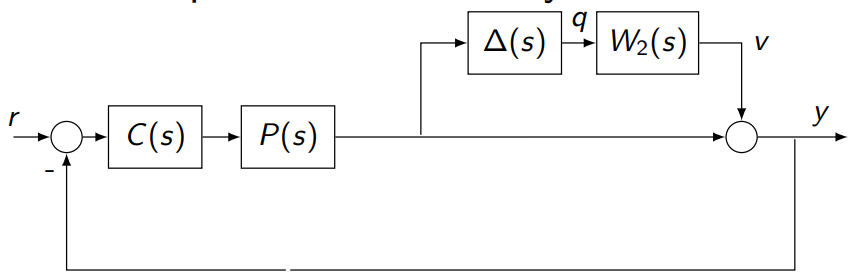
\includegraphics[width = \linewidth]{src/images/uncertainty_block_diagram.png}
    \begin{minipage}{0.58\linewidth}
        \begin{align*}
            \tilde L(s) = (1 + W_2(s) \Delta(s)) P(s) C(s)\\
            L(s) = P(s) C(s)\\
            \Rightarrow |\tilde L(s) - L(s)|\\
            = |W_2(s) \Delta(s) L(s)| \leq |W_2(s) L(s)|
        \end{align*}
        For $\tilde L$ not to encircle the -1 point, Nyquist plot of $L$ should never get closer than $|W_2(s) L(s)$ to -1 point:
        \begin{align*}
            |L(s) + 1| > |W_2(s) L(s)|
        \end{align*}
    \end{minipage}
    \begin{minipage}{0.40\linewidth}
        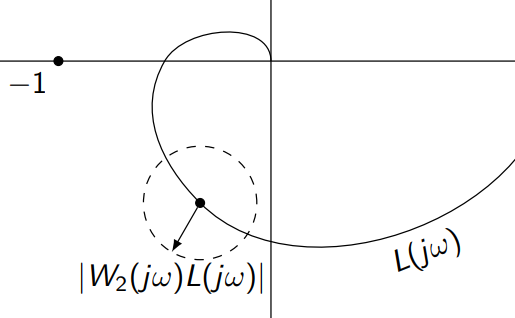
\includegraphics[width = \linewidth]{src/images/uncertainty_nyquist.png}
    \end{minipage}